\section{Tutorial}\label{sec:tutorial}
\subsection{Before the simulation: what to do}\label{subsec:before}
Let us see in practice what we have previously learnt in a simple tutorial:
first of all, we need the whole program, available at \url{https://github.com/BFSteam/memory.}\\
Once downloaded it is convenient to put \texttt{path\_to/memory/src} inside
\texttt{path\_to\_SLAPP3/project.txt} as described in \textit{SLAPP\_Reference\_Handbook.pdf pag20}.
Inside SLAPP3 we can run the program \texttt{runShell.py} from terminal
or from jupyter notebook using \texttt{iRunShell.py}.

The program asks which project we want to run: if we set up the path correctly
we can confirm \textit{memory} path and project.
Afterwards we have to set all the necessary input variables to start
the simulation:
\begin{itemize}
\item[\texttt{Random number seed:}] insert the seed to make the simulation reproducible.
\item[\texttt{Number of sources:}]insert the number of sources inside the network.
\item[\texttt{Number of users:}]insert the number of users inside the network.
\item[\texttt{Average degree for users:}]insert the value of the average degree for users only.
\item[\texttt{Number of cycles:}]insert the maximum number time can reach.
\end{itemize}

In order to simplify our first approach, default values are provided:
answering enter at each line will mak the program run, and that's it!\\

\subsection{During the simulation: where to put the accent}\label{subsec:during}
Simulation is running and our network is evolving. A window will appear
with the drawing network\footnote{Graphs drawn using
  \href{https://networkx.github.io/}{networkx} and
  \href{https://matplotlib.org/}{matplotlib}}
and flowing time is displayed in terminal. \\
Nodes of the network are painted with different colors: if they don't
spread, gray for inactive state and blue for active one; if they spread,
they can be orange, pink or cyan depending on the spread news.
In detail, every source initially generates a single news, tracked by its color. Sources are bigger than users and labeled with 0,1 and 2; numbering goes on with users.\\
We can show network dynamic in the pictures below:
\begin{figure}[!h]
  \centering
  \begin{subfigure}[t]{.45\textwidth}
    \centering
    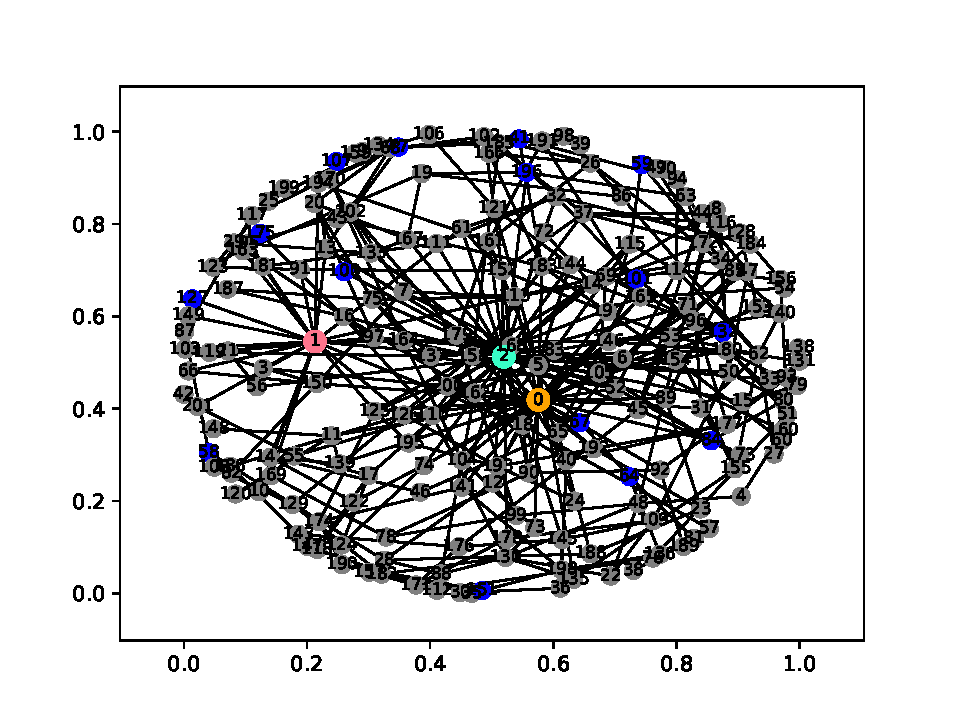
\includegraphics[trim={1cm .5cm 1cm 1cm}, clip, width=\linewidth]{img/pdf/plot-0001.pdf} 
    \caption{1 cycle}
    \label{fig:1}
  \end{subfigure}
  \begin{subfigure}[t]{.45\textwidth}
    \centering
    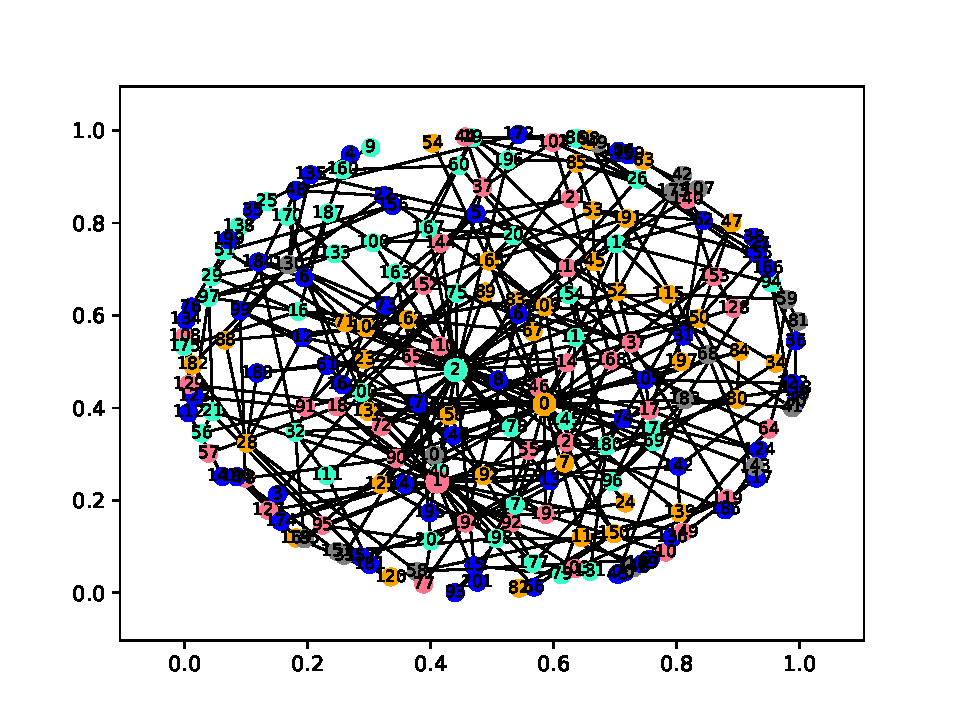
\includegraphics[trim={1cm .5cm 1cm 1cm}, clip, width=\linewidth]{img/pdf/plot-0005.pdf} 
    \caption{5 cycles}
    \label{fig:5}
  \end{subfigure}

  \vspace{0cm}

  \begin{subfigure}[t]{.45\textwidth}
    \centering
    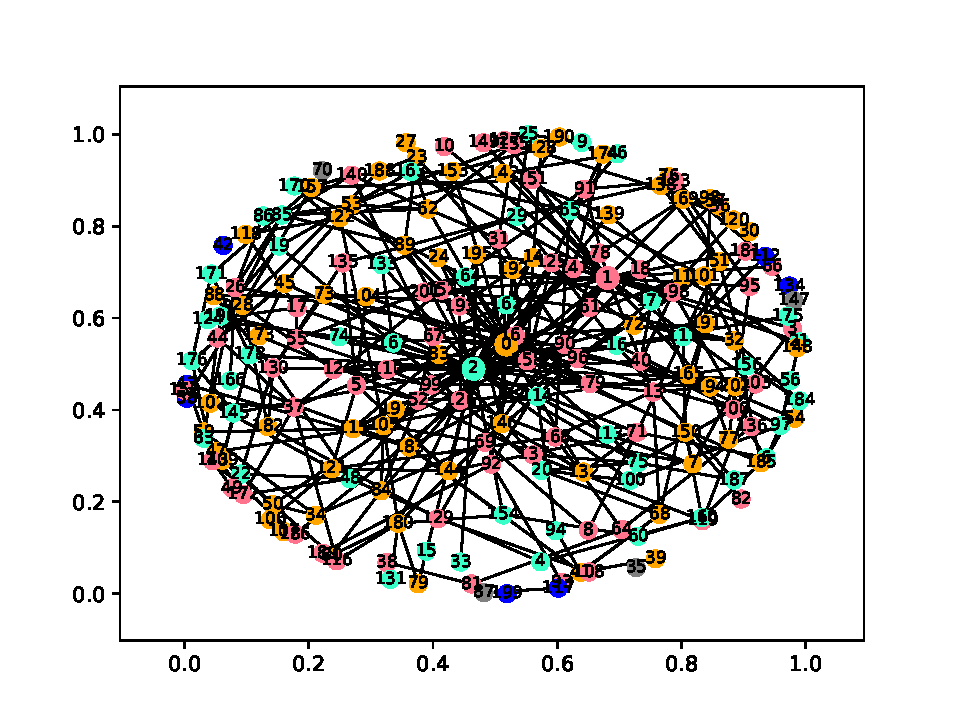
\includegraphics[trim={1cm .5cm 1cm 1cm}, clip, width=\linewidth]{img/pdf/plot-0010.pdf} 
    \caption{10 cycles}
    \label{fig:10}
  \end{subfigure}
  \begin{subfigure}[t]{.45\textwidth}
    \centering
    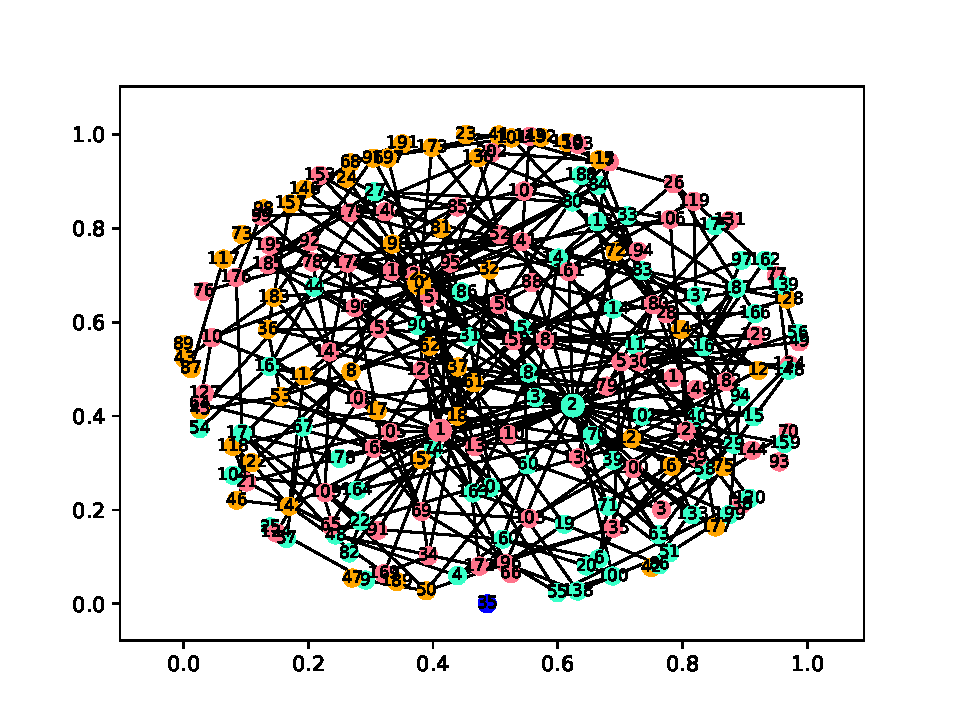
\includegraphics[trim={1cm .5cm 1cm 1cm}, clip, width=\linewidth]{img/pdf/plot-0050.pdf} 
    \caption{50 cycles}
    \label{fig:50}
  \end{subfigure}
 
  \caption{Plot at different time steps for a simulation with 3 sources, 200 users, initial average degree of users 3 and 500 time steps. Random seed initialized to 17}
\end{figure}

\begin{figure}
  \centering
  \begin{subfigure}[t]{.45\textwidth}
    \centering
    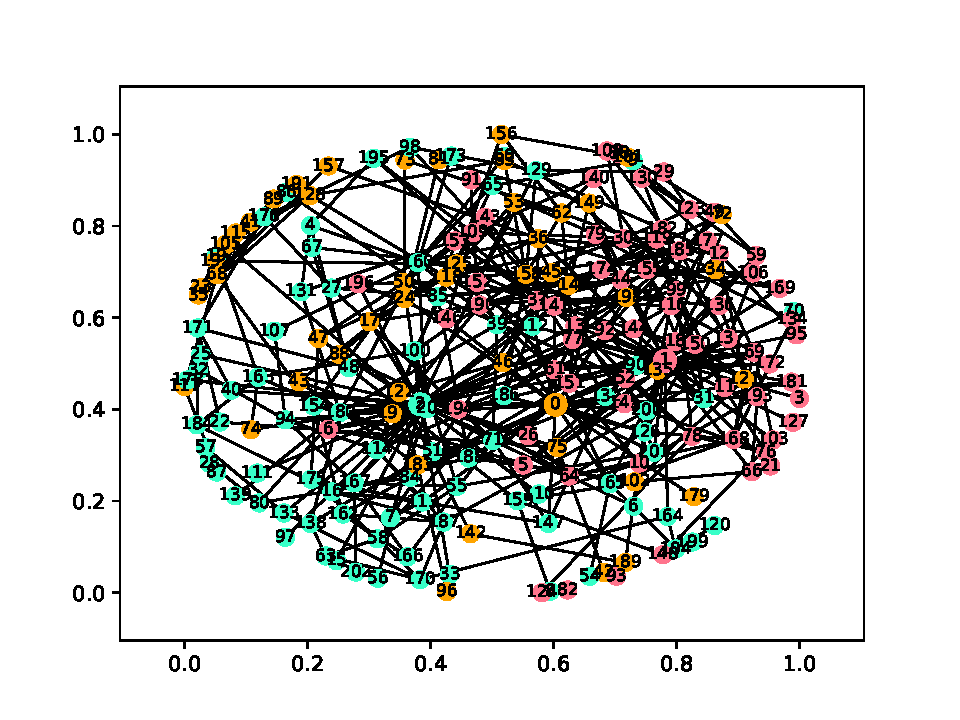
\includegraphics[trim={1cm .5cm 1cm 1cm}, clip, width=\linewidth]{img/pdf/plot-0100.pdf} 
    \caption{100 cycles}
    \label{fig:100}
  \end{subfigure}
  \begin{subfigure}[t]{.45\textwidth}
    \centering
    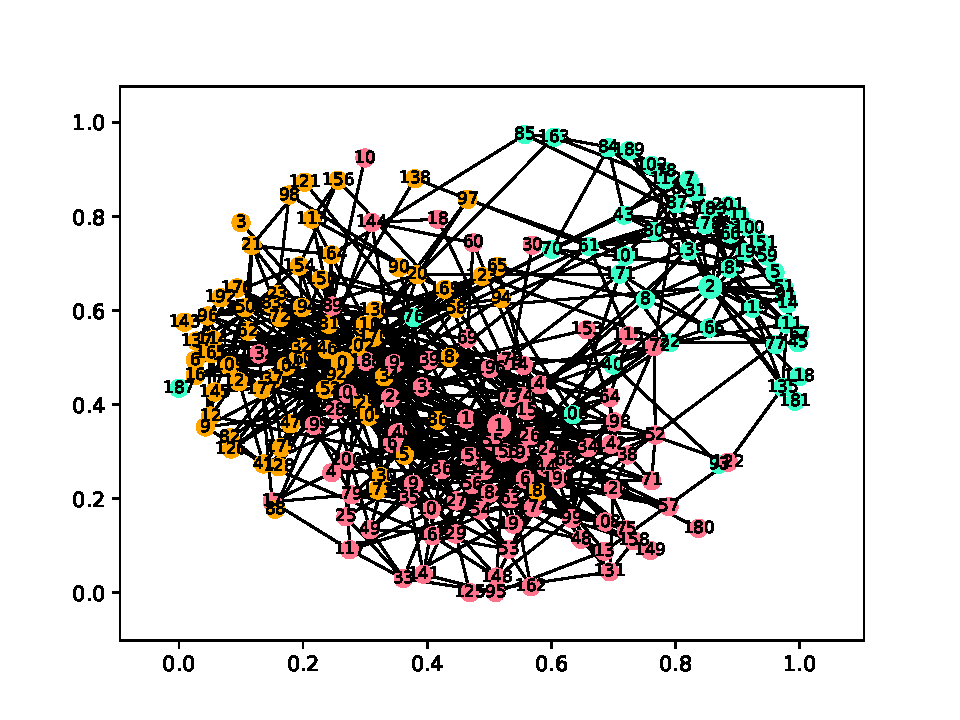
\includegraphics[trim={1cm .5cm 1cm 1cm}, clip, width=\linewidth]{img/pdf/plot-0200.pdf} 
    \caption{200 cycles}
    \label{fig:200}
  \end{subfigure}

  \vspace{0cm}

  \begin{subfigure}[t]{.45\textwidth}
    \centering
    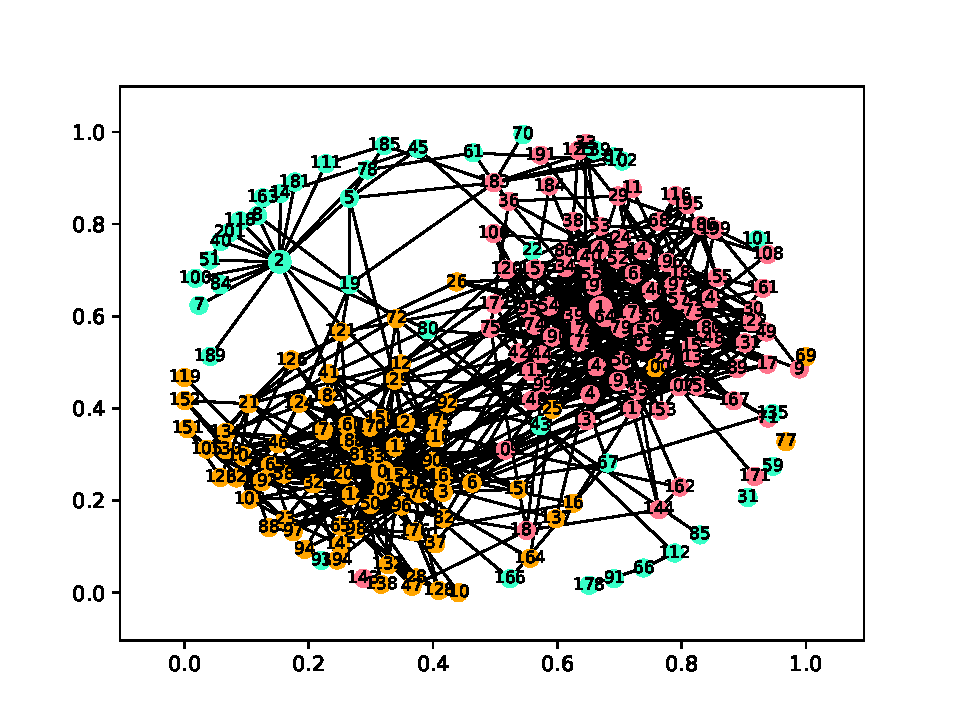
\includegraphics[trim={1cm .5cm 1cm 1cm}, clip, width=\linewidth]{img/pdf/plot-0400.pdf} 
    \caption{400 cycles}
    \label{fig:400}
  \end{subfigure}
  \begin{subfigure}[t]{.45\textwidth}
    \centering
    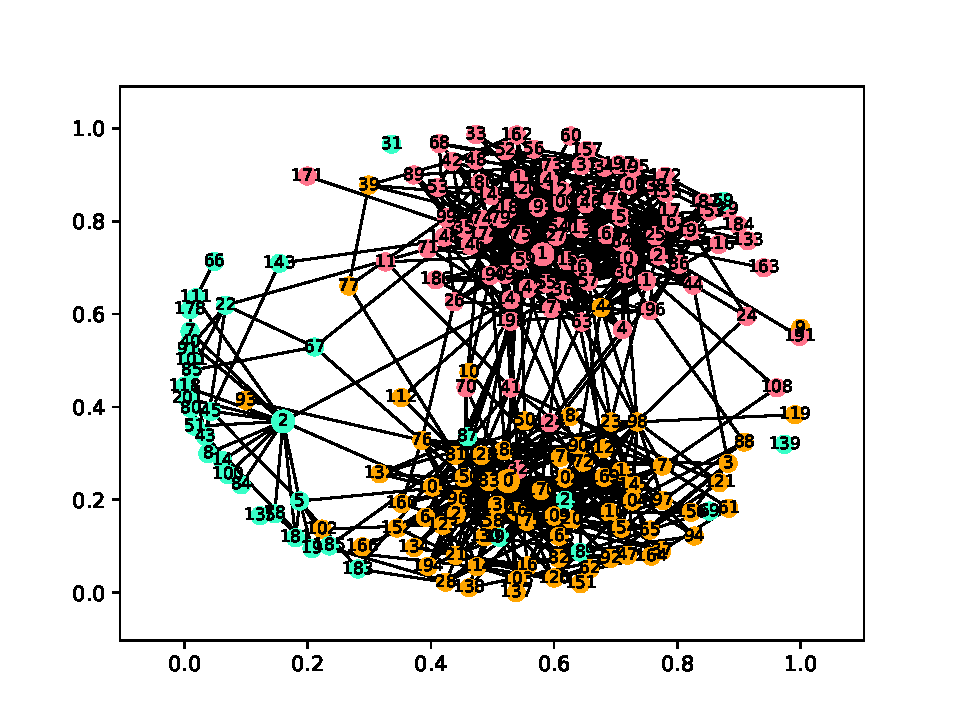
\includegraphics[trim={1cm .5cm 1cm 1cm}, clip, width=\linewidth]{img/pdf/plot-0500.pdf} 
    \caption{500 cycles}
    \label{fig:500}
  \end{subfigure}
 
  \caption{Plot at different time steps for a simulation with 3 sources, 200 users, initial average degree of users 3 and 500 time steps. Random seed initialized to 17}
\end{figure}

\subsection{After the simulation: what to notice}\label{subsec:after}
In figure~\ref{fig:1} we see the net at initialization. Users are mostly
inactive and sources have create one news each. The news are tracked by a
color during the simulation.
After five time steps (figure~\ref{fig:5}) some users have changed their state
to active and started to spread.

\subsection{Further implementations}\label{subsec:implementations}
Some possible future features are:
\begin{itemize}
\item [adding and removing nodes during execution] can yield big changes
  in the process;
\item [look for emerging network behaviors] as said in \textit{\nameref{sec:introduction}} we hope to point out scale-free regime;
\item [analyze the activation time] starting from microscopic behaviors
  it is possible to reproduce macroscopic phenomena such as bursty
  patterns\cite{goh_burstiness_2008}
\end{itemize}

\subsection{Conclusion}\label{subsec:conclusion}







